\documentclass{article}
\usepackage{tikz}
\usetikzlibrary{
	knots,
	hobby,
	decorations.pathreplacing,
	shapes.geometric,
	calc
}

\tikzset{
	knot diagram/every strand/.append style={
		ultra thick,
		red
	},
	show curve controls/.style={
		postaction=decorate,
		decoration={show path construction,
			curveto code={
				\draw [blue, dashed]
				(\tikzinputsegmentfirst) -- (\tikzinputsegmentsupporta)
				node [at end, draw, solid, red, inner sep=2pt]{};
				\draw [blue, dashed]
				(\tikzinputsegmentsupportb) -- (\tikzinputsegmentlast)
				node [at start, draw, solid, red, inner sep=2pt]{}
				node [at end, fill, blue, ellipse, inner sep=2pt]{}
				;
			}
		}
	},
	show curve endpoints/.style={
		postaction=decorate,
		decoration={show path construction,
			curveto code={
				\node [fill, blue, ellipse, inner sep=2pt] at (\tikzinputsegmentlast) {}
				;
			}
		}
	}
}

\title{Nusos}
\author{Guillem Tutusaus i Alcaraz}
\date{March 2024}


%%%%%% Estil del primer dibuix on les curves estan dibuixades intermitentment
\tikzset{
	my style/.style={
		dashed
	}
}

\begin{document}
	
	\maketitle
	
	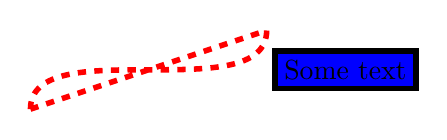
\begin{tikzpicture}[line width=2pt] %%%%%%%%% LÍNIA DISCONTÍNUA
		\draw[my style,red] (0,0) -- (3,1) .. controls +(0,-1) and +(0,1) .. (0,0);
		\node[draw,fill=blue] at (4,.5) {Some text};
	\end{tikzpicture}
	
	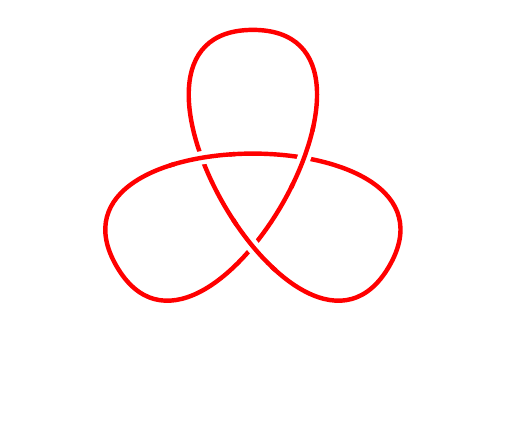
\begin{tikzpicture} %%%%%%%%%%% TREFOIL
		\begin{knot}[
			consider self intersections=true,
			%  draft mode=crossings,
			flip crossing=2,
			only when rendering/.style={
				%    show curve controls
			}
			]
			\strand (0,2) .. controls +(2.2,0) and +(120:-2.2) .. (210:2) .. controls +(120:2.2) and +(60:2.2) .. (-30:2) .. controls +(60:-2.2) and +(-2.2,0) .. (0,2);
		\end{knot}
	\end{tikzpicture}
	
	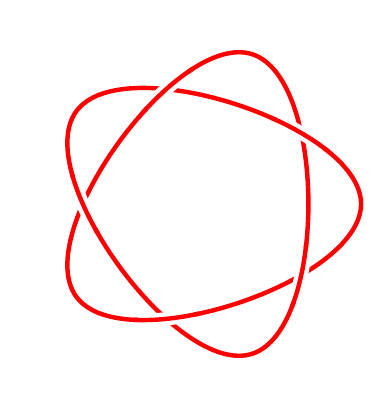
\begin{tikzpicture} %%%%%%%%% PENTÀGON
		\begin{knot}[
			consider self intersections=true,
			%  draft mode=crossings,
			flip crossing/.list={2,4},
			only when rendering/.style={
				%    show curve controls
			}
			]
			\strand (2,0) .. controls +(0,1.0) and +(54:1.0) .. (144:2) .. controls +(54:-1.0) and +(18:-1.0) .. (-72:2) .. controls +(18:1.0) and +(162:-1.0) .. (72:2) .. controls +(162:1.0) and +(126:1.0) .. (-144:2) .. controls +(126:-1.0) and +(0,-1.0) .. (2,0);
		\end{knot}
	\end{tikzpicture}
	
	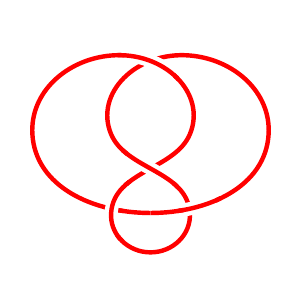
\begin{tikzpicture}[use Hobby shortcut] %%%%%%%% VUIT
		\begin{knot}[
			consider self intersections=true,
			%draft mode=crossings,
			ignore endpoint intersections=false,
			flip crossing/.list={3,4},
			only when rendering/.style={
			%show curve endpoints
			}
			]
			\strand ([closed]0,0) .. (1.5,1) .. (.5,2) .. (-.5,1) .. (.5,0) .. (0,-.5) .. (-.5,0) .. (.5,1) .. (-.5,2) .. (-1.5,1) .. (0,0);
		\end{knot}
		\path (0,-.7);
	\end{tikzpicture}
	
	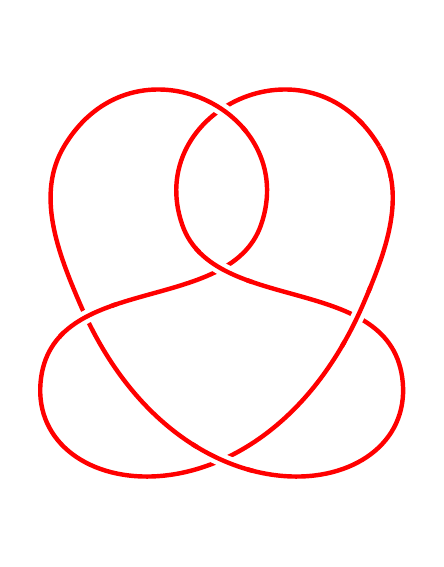
\begin{tikzpicture}[use Hobby shortcut] %%%%% 5 CREUAMENTS
		\begin{knot}[
			consider self intersections=true,
			%  draft mode=crossings,
			ignore endpoint intersections=false,
			flip crossing/.list={6,4,2}
			]
			\strand ([closed]2,2) .. (1.8,0) .. (-2.3,-1) .. (.5,1) .. (-2,2) .. (-1.8,0) .. (2.3,-1) .. (-.5,1) .. (2,2);
		\end{knot}
	\end{tikzpicture}
	
	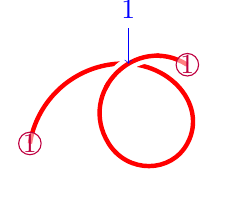
\begin{tikzpicture}[use Hobby shortcut] %%%%% FIGURA AMB NÚMEROS 1'S
		\begin{knot}[
			consider self intersections=true,
			draft mode=crossings,
			ignore endpoint intersections=false,
			flip crossing=1
			]
			\strand (0,0) .. (1,1) .. (2,0) .. (1,0) .. (2,1);
		\end{knot}
	\end{tikzpicture}
	
	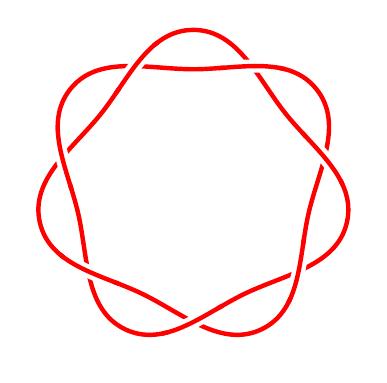
\begin{tikzpicture}[use Hobby shortcut] %%%% HEPTÀGON
		\begin{knot}[
			consider self intersections=true,
			%  draft mode=crossings,
			flip crossing/.list={2,4,6}
			]
			\strand ([closed]90:2) foreach \k in {1,...,7} { .. (90-360/7+\k*720/7:1.5) .. (90+\k*720/7:2) } (90:2);
		\end{knot}
	\end{tikzpicture}
	
	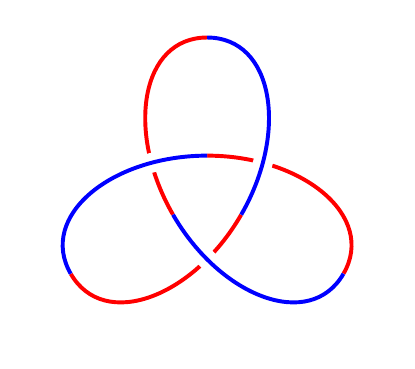
\begin{tikzpicture}[ %%%%%%%% TREFOIL DE COLORS
		use Hobby shortcut,
		every path/.style={
			line width=1mm,
			white,
			double=red,
			double distance=.5mm
		}
		]
		\def\nfoil{3}
		\draw ([closed]0,2)
		foreach \k in {1,...,\nfoil} {
			.. ([blank=soft]90+360*\k/\nfoil-180/\nfoil:-.5) .. (90+360*\k/\nfoil:2)
		};
		\draw[use previous Hobby path={invert soft blanks,disjoint},double=blue];
	\end{tikzpicture}
	
\end{document}
